\chapter{Methodology} \label{ch:methodology}

	The \toolname\ provides several features: \textit{(i)} phase of flight identification, \textit{(ii)} quality analysis of each phase, \textit{(iii)} grade assignment, and \textit{(iv)} a web interface to display results.  Since there are three separate phases of concern, there will be a separate subsection for each in both identification and quality analysis.  These features are discussed in more detail in the rest of this chapter.

%----------------------------------------
% PHASE IDENTIFICATION
%----------------------------------------
\section{Phase of Flight Identification}

\note{Not trivial because multiple circuits in a single flight. Lack technology found in commercial aircraft. Flying patterns are highly variable in GA due to flight training.}

	%----------
    % APPROACH
    %----------
	\subsection{Approach}
    
    	The Approach phase is defined as the time between the aircraft entering the airport's traffic pattern (shown in \Cref{fig:traffic_pattern}), or 1,000 feet above the runway elevation, to the beginning of the landing flare under Visual Flight Rules (VFR).  For Instrument Flight Rules (IFR), it is the time from the Initial Approach Fix (IAF) to the beginning of the landing flare~\cite{cictt2013phase}.
        
        \begin{figure}
        	\centering
            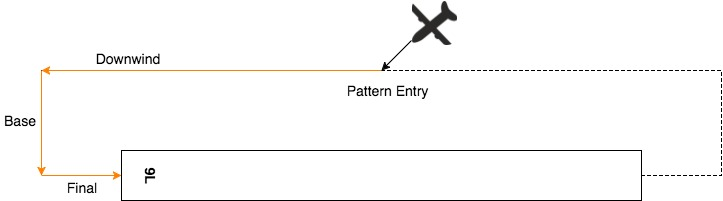
\includegraphics[width=\linewidth]{img/airport_traffic_pattern.jpg}
            \caption{Example showing an airport's traffic pattern and the subphases of the Approach.}
            \label{fig:traffic_pattern}
        \end{figure}
        
    
    %----------
    % LANDING
    %----------
    \subsection{Landing}
    
    The Landing phase is defined as the time from the beginning of the landing flare until the aircraft performs one of the following actions: \textit{(i)} exits the landing runway, \textit{(ii)}, comes to a complete stop on the runway (full-stop), or \textit{(iii)} when power is applied for takeoff in the case of a touch-and-go landing~\cite{cictt2013phase}.
    
    
    %----------
    % TAKEOFF
    %----------
    \subsection{Takeoff}
    
    The Takeoff phase is defined as the time from the application of takeoff power, through rotation, and to an altitude of 35 feet above the runway elevation~\cite{cictt2013phase}.
    

%----------------------------------------
% PHASE QUALITY ANALYSIS
%----------------------------------------
\section{Phase of Flight Quality Analysis \& Exceedance Detection}
    
    %----------
    % APPROACH
    %----------
	\subsection{Approach}
    	\note{Includes turn-to-final, stabilized parameters, self-defined}
    
    
    %----------
    % LANDING
    %----------
    \subsection{Landing}
    
    
    %----------
    % TAKEOFF
    %----------
    \subsection{Takeoff}
    	\note{stabilized parameters}
    

%----------------------------------------
% GRADING METRICS
%----------------------------------------
\section{Grading Metrics}

	\note{previous expert knowledge, how do different possible error metrics overlap?, use standard deviations?}
    
    
%----------------------------------------
% WEB INTERFACE
%----------------------------------------
\section{Web Interface}

	\note{Not sure if I'll keep this section here? Might just mention libraries used in Implementation section, then show screenshots in results.}

